\documentclass{article}
\usepackage{graphicx}

\title{A Lanyard Puzzle}
\author{Cecilia Sun}

\begin{document}

\maketitle
%\begin{center}
%    \includegraphics[scale=0.6]{img/Vol2/lanyard11.png}
%\end{center}
%removing for spacing reasons

Recently, I spent 5 weeks at Canada/USA Mathcamp. Being surrounded by math kids, our mealtime chatter frequently included spirited conversations about some interesting math puzzle or problem. Out of all the problems we pondered, one of the puzzles that caused the most lively dinnertime discussions was what we called the lanyard puzzle. It’s most commonly known as the Picture-Hanging puzzle, but, being at camp and having an abundance of lanyards (we each had one to hang the various keys and cards given to us by the university), we called it the lanyard puzzle. 

The most simple formation of the puzzle is as follows: suppose you have two pegs, and you want to hang the lanyard around these pegs such that removing either peg causes the lanyard to fall. Is this possible? If so, how? 

If you spend some time experimenting, you might come up with the following configuration, which is indeed a solution to the puzzle:

\begin{center}
    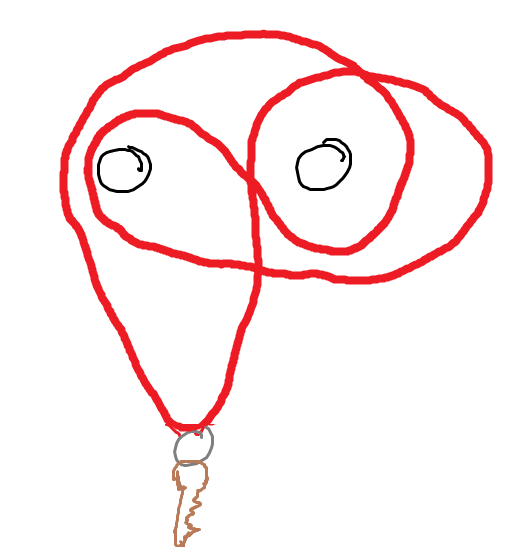
\includegraphics[scale=0.4]{images/lanyard2.png}
\end{center}

After finding this solution, you might be inclined to see if we can generalize this to more pegs: for instance, can we hang a lanyard from three pegs such that removing any singular peg causes the lanyard to fall? What about four pegs? $n$ pegs? As it turns out, the answer is yes, but to see this we first return to the two-peg case to see what is really going on. 

Firstly, let's name our pegs $A$ and $B$. 

\begin{center}
    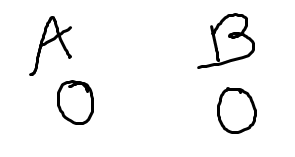
\includegraphics[scale = 0.6]{images/lanyard3.png}
\end{center}

Observe that, while hanging the lanyard, we only really have four distinct moves: wrapping the lanyard around peg $A$ clockwise, wrapping it around peg $A$ counterclockwise, wrapping it around peg $B$ clockwise, and wrapping it around peg $B$ counterclockwise. Let’s call these operations $A$, $A’$, $B$, and $B’$ respectively. Thus, we can express each hanging configuration as a string of these four operations. 

\begin{center}
    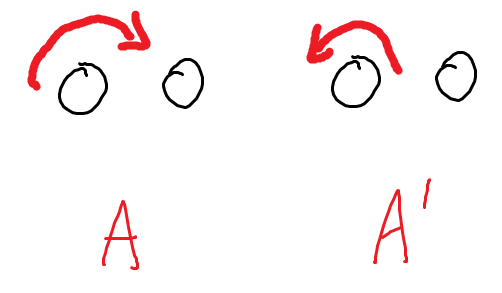
\includegraphics[scale=0.4]{images/lanyard41.png}
    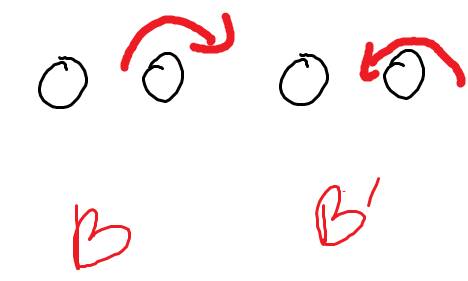
\includegraphics[scale=0.4]{images/lanyard42.png}
\end{center}

From here we make two observations:

Firstly, if we ever have $A$ and $A’$ right next to each other, they cancel each other out. The same applies to $B$ and $B’$.

%\begin{center}
%    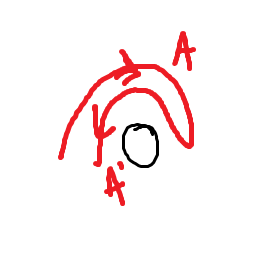
\includegraphics[scale=0.6]{images/lanyard5.png}
%\end{center}

Secondly, removing a peg removes all operations associated with that peg from the string. So, removing peg $A$ will cause all instances of operation $A$ or $A’$ to be removed from the string. 

If we look at our solution, we can write out the sequence of operations it’s associated with: 

\begin{center}
    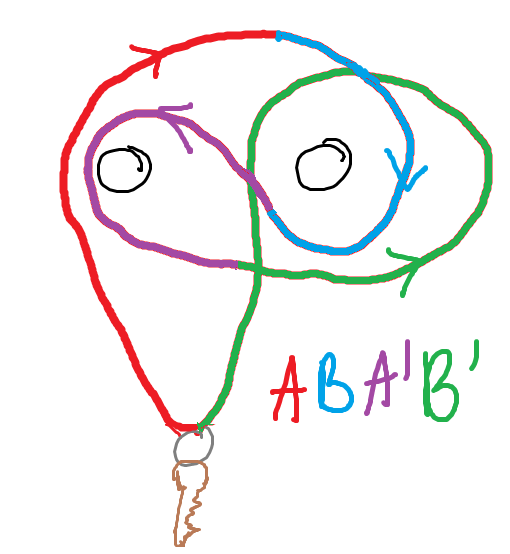
\includegraphics[scale=0.4]{images/lanyard6.png}
\end{center}

Note that removing all the $B$’s will reduce the sequence to $AA’$ which cancels into nothing, meaning the lanyard drops; the same is true for removing the $A$’s.

From here, we have a sufficient framework to examine cases in which there are more pegs.

Firstly, for notational ease, let's rename the pegs to pegs $1$, $2$, $3$, $\dots$. We denote hanging the lanyard clockwise around peg $n$ to be $x_n$, and hanging the lanyard counterclockwise around peg $n$ to be $x_n^{-1}$ (under this notation, it is also clearer that looping clockwise and counterclockwise around the same peg are ``inverse" operations). Let's also let $S_n$ denote the sequence of operations around the first $n$ pegs that causes the lanyard to drop upon removing any of the first $n$ pegs. So, $S_2=x_1x_2x_1^{-1}x_2^{-1}$ and we want to find $S_3$.

Our work for the $2$-peg case is actually useful here! If, for example, we put $S_2$ ``between" $x_3$ and its inverse, $x_3^{-1}$, then removing either $A$ or $B$ will cause $S_2$ to cancel out, after which the $x_3$ and $x_3^{-1}$ will be next to each other and cancel each other out.

But we run into an issue when peg 3 is removed -- the string becomes $S_2$, which does not fall off the peg! If we find a configuration (which we will call $S_2^{-1}$) to put after the $x_3^{-1}$ such that $S_2S_2^{-1}$ cancels out, then we win! 
It turns out that we can just directly do this; we start at the last operation in $S_2$ and take its inverse, then continue appending the inverse of the operation from right to left until we reach the end.

For example, to invert $x_1x_2x_1^{-1}x_2^{-1}$, we start at the right end, with the inverse of $x_2^{-1}$ (which is just $x_2$). Then we go to the next operation (moving left) with the inverse of $x_1^{-1}$ (so, our string is now $x_2x_1$); eventually, we end up with $S_2^{-1}=x_2x_1x_2^{-1}x_1^{-1}$. 

We can also check that $S_2S_2^{-1}$ completely cancels out:

\begin{align*}
	S_2S_2^{-1}&= x_1x_2x_1^{-1}x_2^{-1}x_2x_1x_2^{-1}x_1^{-1} \\
	&= x_1x_2x_1^{-1}(x_2^{-1}x_2)x_1x_2^{-1}x_1^{-1} \\
	&= x_1x_2x_1^{-1}x_1x_2^{-1}x_1^{-1} \\
	&= x_1x_2(x_1^{-1}x_1)x_2^{-1}x_1^{-1} \\
	&= x_1x_2x_2^{-1}x_1^{-1} \\
	&= x_1(x_2x_2^{-1})x_1^{-1} \\
	&= x_1x_1^{-1}
\end{align*}

Now that we have verified that $S_2^{-1}$ does indeed exist, we arrive at the final construction $S_3=S_2x_3S_2^{-1}x_3^{-1}=x_1x_2x_1^{-1}x_2^{-1}x_3x_2x_1x_2^{-1}x_1^{-1}x_3^{-1}$.

\begin{center}
    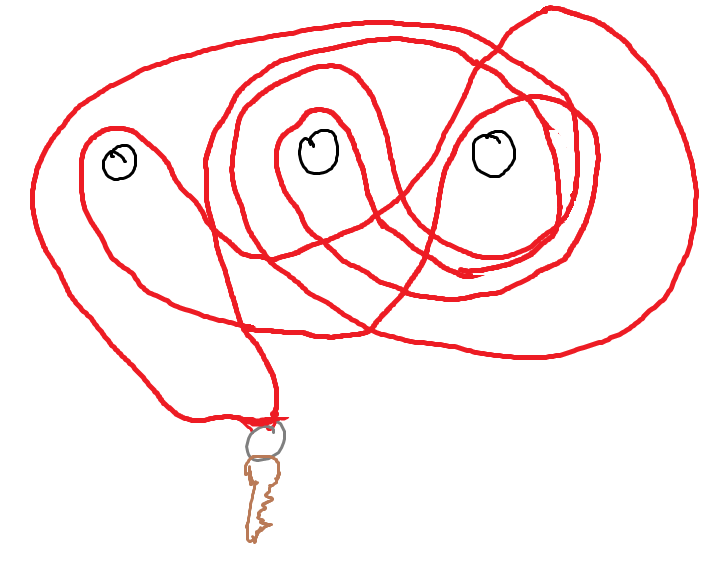
\includegraphics[scale = 0.4]{images/lanyard71.png}
\end{center}

We can, in fact, generalize this to any number of pegs; for $S_4$ we can take $S_3x_4S_3^{-1}x_4^{-1}$ to get the extremely lengthy construction
$S_4=x_1x_2x_1^{-1}x_2^{-1}x_3x_2x_1x_2^{-1}x_1^{-1}x_3^{-1}x_4x_3x_1$ $x_2x_1^{-1}x_2^{-1}x_3^{-1}x_2x_1x_2^{-1}x_1^{-1}x_4^{-1}$. To get $S_n$ we can take $S_{n-1}x_nS_{n-1}^{-1}x_n^{-1}$. This is what we call a \textit{recursive construction}, since our construction for $n$ pegs depends on the construction for $n-1$ pegs. 
So, it turns out for \textbf{any number of pegs} there always exists a way to wrap a lanyard around all the pegs such that the picture hangs when all the pegs are intact, but drops once any single peg is removed---we just might need a really long string!

At this point, my friends and I had solved the puzzle (and finished our dinners), but we weren’t quite satisfied yet, due to a small issue -- we could easily demonstrate the 2-peg configuration by wrapping our lanyards around our fingers; the 3-peg configuration was trickier because it had more operations and thus required a lot more wrapping, but once we got to 4 pegs the lanyard was simply too short and the number of operations (22) too large to demonstrate it physically.

Our construction is indeed pretty inefficient in terms of the number of operations in each $S_n$; in fact, each time we add a new peg, we more than double the number of operations (since we include a copy of both $S_{n-1}$ \textbf{and} $S_{n-1}^{-1}$); the number of operations is growing exponentially under this construction!

However, it turns out that there is a more efficient way to recursively build up $S_n$. The key idea is to keep the format 

The idea is to keep the $ABA^{-1}B^{-1}$ format, but instead try to have $A$ and $B$ be more balanced. Instead of having one of $A$ and $B$ account for just one peg and the other account for all the rest of the pegs, we split the pegs into two groups as evenly as we can and have $A$ account for the first group of pegs (in other words, $A$ will be the sequence for which removing any single peg within the first group of pegs will completely cancel $A$ out) and $B$ account for the second group of pegs. This way, instead of constructing $S_n$ in terms of $S_1$ and $S_{n-1}$ we instead construct it in terms of $S_{\lfloor n/2\rfloor}$ and $S_{\lceil n/2 \rceil}$. 

\begin{center}
    
\includegraphics[scale = 0.8]{images/lanyard1.png}
\end{center}
\end{document}